%%%%%%%%%%%%%%%%%%%%%%%%%%%%%%%%%%%%%%%%%%%%%%%%
% 1: Introducción
%%%%%%%%%%%%%%%%%%%%%%%%%%%%%%%%%%%%%%%%%%%%%%%%
\pagenumbering{arabic} % para empezar la numeración con números
\chapter{Introducción}\label{introduccion}

Como dice Maude Lemaire en \cite{lemaire2014incorporating}, en una sociedad que está incrementando su dependencia a las nuevas tecnologías\footnote{Aquí, con nuevas tecnologías me refiero a productos y proyectos derivados de la Informática y las \acrfull{TIC} como puede ser los proyectos que detallamos en la sección \ref{estado-arte}.}, es imprescindible que las nuevas generaciones desarrollen la habilidad de pensar de manera crítica sobre tecnología.



%In a society becoming increasingly dependent on software, it is imperative that our younger generation develop the ability to think critically about technol- ogy. With a resounding push for engineering education in recent years, the availability of computer science education to students of all levels has been a growing discussion at educational ministries within the government of nu- merous industrialized nations, particularly in France and the United Kingdom [2]. The movement has led to the development of dozens of online platforms dedicated to educating children levels K-12 and beyond, including Codecademy (www.codecademy.com), CodeHS (www.codehs.com), Code.org (www.code.org), Scratch (scratch.mit.edu), and Alice (www.alice.org) [6]. Available in multiple languages and to anyone with an Internet connection, many of these websites of- fer content for teachers wishing to integrate programming into their classrooms;




\section{Aprendizaje usando herramientas informáticas}
\label{sec:aprendizaje}

\subsection{Aprendiendo a programar}
\label{sub:aprendiendo-programar}

\section{Descubre}
\label{sec:descubre}


\section{Motivación y enfoque del proyecto}
\label{sec:motivacion}


%%%%%%%%%%%%%%%%%%%%%%%%%%%%%%%%%%%%%%%%%%%%%%%%
% 2: Estado del arte
%%%%%%%%%%%%%%%%%%%%%%%%%%%%%%%%%%%%%%%%%%%%%%%%
\chapter{Estado del arte}\label{estado-arte}



A nivel global, actualmente existe una gran cantidad de proyectos con la única intención de enseñar, principalmente a algumos de secundaria y bachillerato, diferentes aspectos de la informática como lo es la programación \cite{code-school,code-org,code-academy}, la robótica \cite{robomind-web,moway} e incluso chips y electrónica con \Gls{arduino}\cite{arduino}. Algunos de estos proyectos llevan décadas activos, como lo es el lenguaje \Gls{logo}\cite{logo} y su proyecto \Gls{turtle}\cite{logo-turtle}
La mayoría de estos proyectos promueven una enseñanza independiente y autodidacta bajo un entorno on-line. De esta manera, el alumno puede aprender a su propio ritmo y desde cualquier parte del mundo.


\section{El lenguaje Logo y el robot Turtle}
\label{sec:Logo}

El lenguaje Logo, basado en \Gls{lisp}, fue diseñado como una herramienta para aprendizaje. Todas sus características -interactividad, modularidad, extensibilidad, flexibilidad en los tipos de datos- persiguen esta meta.

%The Logo Programming Language, a dialect of Lisp, was designed as a tool for learning. Its features - interactivity, modularity, extensibility, flexibility of data types - follow from this goal.

Como se explica en la página oficial del proyecto Logo\cite{logo}, durante la década de los 70, en el \acrfull{MIT} y diferentes centros de investigación europeos, se llevó a cabo una investigación sobre el uso del \Gls{logo} en un pequeño grupo de alumnos de secundaria. Todo el proceso se ha documentado en diferentes artículos como \cite{feurzeig1969programming} o \cite{pea1984logo}.

%Throughout the 1970s Logo was incubating at MIT and a few other research sites: Edinburgh, Scotland and Tasmania, Australia. There were small research activities conducted in local schools, including the Brookline Public Schools, just up the Charles River from MIT. Dan Watt, Cynthia Solomon, and other MIT researchers documented their work with a small number of elementary school students using Logo. Their reports are among the several dozen Logo Memos published by MIT during this period.

El proyecto Turtle es el proyecto más popular del lenguaje Logo. Nació como una criatura robótica que se movía por el suelo y se podía programar solo con 2 instrucciones básicas: \texttt{forward x} y \texttt{right y}, para avanzar \texttt{x} \emph{pasos de tortuga} o girar \texttt{y} grados hacia la derecha, respectivamente.

Combinando estas dos instrucciones de lo más simples, nuestro robot tortuga puede realizar cualquier movimiento más complejo, como podemos ver en la figura \ref{fig:mov-tortle}.

\begin{figure}[!ht]
	\begin{centering}
		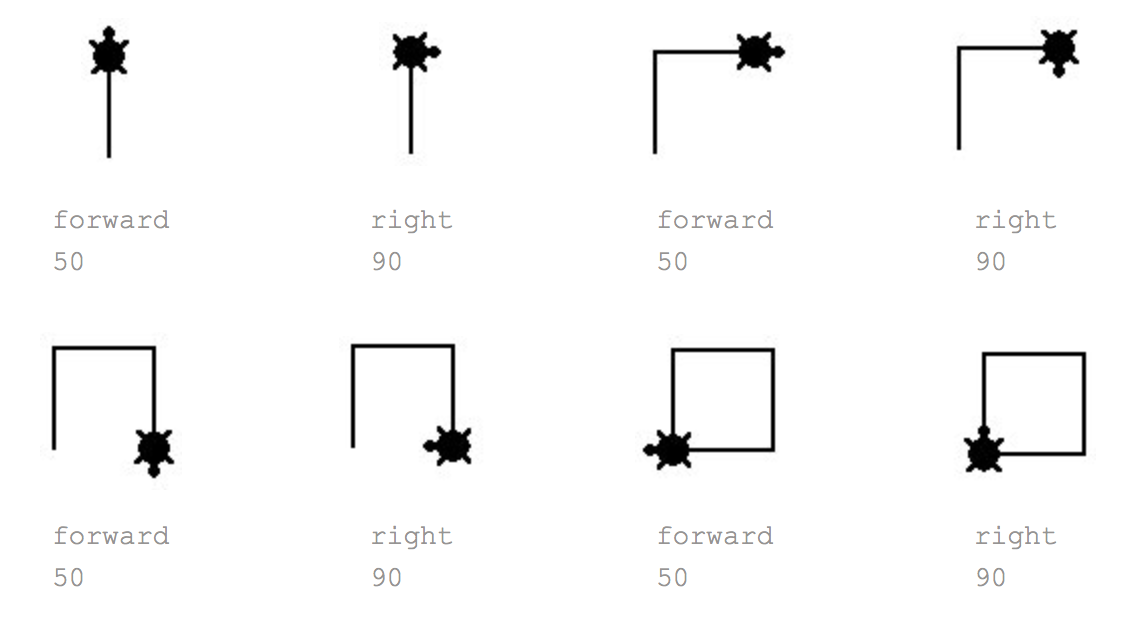
\includegraphics[width=0.8\textwidth]{images/mov-tortle.png}
			\caption{Movimiento de Tortle en forma de cuadrado utilizando unicamente sus instrucciones básicas \texttt{forward} y \texttt{right}.}
				\label{fig:mov-tortle}
	\end{centering}
\end{figure}

Para ilustrar brevemente el lenguaje Logo junto con el robot Turtle, vamos a mostrar como se dibujaría una figura que guarda cierto parecido a una flor.
En el código que se muestra a continuación, creamos una función \texttt{square} que dibuja un cuadrado de tamaño 50 pasos, como podemos ver en la figura \ref{fig:square-turtle}

\begin{lstlisting}
to square
	repeat 4 [forward 50 right 90]
end
\end{lstlisting}

Y a continuación definimos una función \texttt{flower} que utiliza la función \texttt{square} antes descrita y que dibujará una flor, como se puede apreciar en la figura \ref{fig:flower-turtle}

\begin{lstlisting}
to flower
	repeat 36 [right 10 square]
end
\end{lstlisting}

\begin{figure}[!ht]
	\begin{adjustwidth}{\oddsidemargin-1in}{\rightmargin}
	%	\centering
			\begin{subfigure}{\paperwidth}
				\centering
				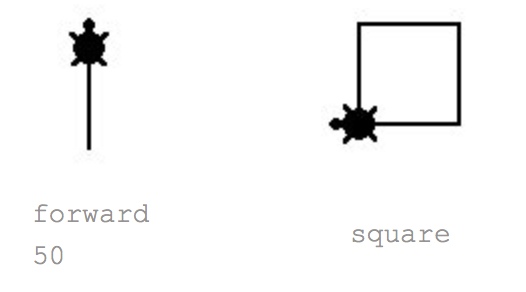
\includegraphics[scale=.45]{images/square-turtle.png}
				\caption{Cuadrado dibujado por el robot Turtle.}
				\label{fig:square-turtle}
			\end{subfigure}
			\begin{subfigure}{\paperwidth}
				\centering
				
\includegraphics[scale=.45]{images/flower-turtle.png}
				\caption{Flor dibujada por el robot Turle.}
				\label{fig:flower-turtle}
			\end{subfigure}
			%\caption{Ejemplo de dibujo utilizando funciones por el robot Turtle.}
		\label{fig:square-flower-turtle}
	\end{adjustwidth}
\end{figure}


El proyecto Tortle ha sido reproducido en proyectos más recientes como \Gls{scratch}\cite{scratch}, el cual se verá en más profundidad en la sección \ref{sec:blockly-scratch}.



\section{Khan Academy}
\label{sec:Khan Academy}

Khan Academy\cite{khan-academy}, con casi 37 millones de usuarios, es uno de los mayores proyectos web para aprender casi de cualquier tema: Matemáticas, estadística, economía o humanidades.


\section{Code.org}
\label{sec:Code.org}

Code.org\cite{code-org} es una plataforma on-line que se dedica exclusivamente a enseñar a programar y cuenta ya con más de 8 millones de usuarios. Cuenta con una gran comunidad de educadores y apoyos entre los que se puede contar al Presidente B. H. Obama. Lleva a cabo proyectos como \emph{Hour of Code} en el que promueve que los usuarios inviertan una hora diaria programando en diferentes juegos, muchos de ellos utilizando \Gls{Blockly}\cite{blockly}.

{\color{red} Parece que estoy haciendo publicidad... shit}


\section{Squeak Etoys}
\label{sec:squeak-etoys}


\section{Blockly y Scratch}
\label{sec:blockly-scratch}


%%%%%%%%%%%%%%%%%%%%%%%%%%%%%%%%%%%%%%%%%%%%%%%%
% 3: Análisis de objetivos y metodología
%%%%%%%%%%%%%%%%%%%%%%%%%%%%%%%%%%%%%%%%%%%%%%%%
\chapter{Análisis de objetivos y metodología}\label{objetivos-metodologia}

\section{Objetivos}
\label{sec:Objetivos}

Este Trabajo Fin de Grado consiste en desarrollar un módulo de simulación de un robot para integrarlo en la plataforma \Gls{descubre}. Para ello se tendrán que cubrir una serie de subobjetivos que nombraremos a continuación.
\begin{itemize}
\item Estudiar el uso y aplicación de diferentes librerías de físicas para generar el robot.
\item Comprensión de la plataforma Descubre así como su posterior modificación.
\item Creación de un simulador de un robot de dos ruedas y su integración en la plataforma Descubre.
\item Modificación del motor de \gls{ijava} y creación de la \acrshort{API} para poder controlar el robot.
\end{itemize}

\section{Metodología}
\label{sec:metodologia}

%%%%%%%%%%%%%%%%%%%%%%%%%%%%%%%%%%%%%%%%%%%%%%%%
% 4: Diseño y resolución del trabajo realizado
%%%%%%%%%%%%%%%%%%%%%%%%%%%%%%%%%%%%%%%%%%%%%%%%
\chapter{Diseño y resolución del trabajo realizado}\label{diseno}




%%%%%%%%%%%%%%%%%%%%%%%%%%%%%%%%%%%%%%%%%%%%%%%%
% 5: Conclusiones y vías futuras
%%%%%%%%%%%%%%%%%%%%%%%%%%%%%%%%%%%%%%%%%%%%%%%%
\chapter{Conclusiones y vías futuras}\label{conslusiones}
